\documentclass[a5paper]{article}
\usepackage[a5paper, top=8mm, bottom=8mm, left=8mm, right=8mm]{geometry}

\usepackage{polyglossia}
\setdefaultlanguage[babelshorthands=true]{russian}

\usepackage{fontspec}
\setmainfont{FreeSerif}
\newfontfamily{\russianfonttt}[Scale=0.7]{DejaVuSansMono}

\usepackage[font=scriptsize]{caption}

\usepackage{amsmath}
\usepackage{amssymb,amsfonts,textcomp}
\usepackage{color}
\usepackage{array}
\usepackage{hhline}
\usepackage{cite}
\usepackage{textcomp}

\usepackage[hang,multiple]{footmisc}
\renewcommand{\footnotelayout}{\raggedright}

\PassOptionsToPackage{hyphens}{url}\usepackage[xetex,linktocpage=true,plainpages=false,pdfpagelabels=false]{hyperref}
\hypersetup{colorlinks=true, linkcolor=blue, citecolor=blue, filecolor=blue, urlcolor=blue, pdftitle=1, pdfauthor=, pdfsubject=, pdfkeywords=}

\newlength\Colsep
\setlength\Colsep{10pt}

\usepackage{tabu}

\usepackage{graphicx}
\usepackage{indentfirst}
\usepackage{multirow}
\usepackage{subfig}
\usepackage{footnote}
\usepackage{minted}

\newcommand{\todo}[1] {
\begin{center}\textcolor{red}{TODO: #1}\end{center}
}

\newcommand{\attribution}[1] {
	\vspace{-5mm}\begin{flushright}\begin{scriptsize}%\textcolor{gray}
	{\textcopyright\, #1}\end{scriptsize}\end{flushright}
}

\sloppy
\pagestyle{plain}

\title{Лекция 9: Антипаттерны}
\author{Юрий Литвинов\\\small{yurii.litvinov@gmail.com}}
\date{}

\begin{document}

\maketitle
\thispagestyle{empty}

\section{Введение}

В этой лекции будет рассказано про то, как делать не надо. В литературе есть термин ``Антипаттерны'', имеющий тот же смысл, что и паттерны, но наоборот: если паттерны --- это часто встречающиеся решения, приводящие к известным преимуществам, то антипаттерны --- это часто встречающиеся решения, приводящие к известным проблемам. Оказывается, что знание антипаттернов для архитектора даже полезнее, чем знание паттернов, поскольку позволяет избежать очень частых и очень дорогостоящих ошибок.

Точно так же, как и паттерны, антипаттерны документируют, чтобы иметь общий словарь (например, не пускаться в пространные рассказы про то, что есть принцип единственности ответственности, что класс, который делает вообще всё --- это плохо, и почему, а просто сказать, что это антипаттерн ``God Object''). Кроме того, описание антипаттерна, помимо описания проблемы и пояснения, почему это плохо, должно по-хорошему содержать и рекомендации по тому, как это исправить. 

Хочется заметить, что антипаттерны часто описывают решения, которые сами по себе неплохи и вполне применяются на практике без всяких проблем, типичный пример --- это ``Busy waiting'', успешно применяющийся в микроконтроллерах. Источником проблем часто является не само решение, а контекст его применения --- например, ``Busy waiting'' может быть очень плохой идеей, если минутами грузит процессор на ноутбуке.

Антипаттерны, так же, как и паттерны, имеют некую классификацию, но не по назначению, а по ``сфере применения'' --- антипаттерны реализации (в том числе, специфичные для конкретного языка или технологии, которые мы в этой лекции затрагивать не будем), архитектурные антипаттерны и организационные антипаттерны (которые мы тоже затрагивать практически не будем, потому что это больше про управление проектами, чем про архитектуру). Мы начнём с антипаттернов реализации и продолжим архитектурными антипаттернами.

\noindent\begin{minipage}{\textwidth}
	\begin{minipage}[c][6cm][c]{\dimexpr0.7\textwidth-0.5\Colsep\relax}
		Дальнейшее изложение будет вестись по книжке AntiPatterns: Refactoring Software, Architectures, and Projects in Crisis by William J. Brown, Raphael C. Malveau, SkipMcCormick, Thomas J. Mowbray, Wiley, 1998, 336pp. Книга столь же старая, что и книга про паттерны, и с момента её издания появилась куча специфичных для языков и технологий антипаттернов, но они нам как раз и не очень интересны. Антипаттерны, касающиеся разработки в целом, за это время нисколько не поменялись. Книга не входит в рекомендованную по этому курсу литературу, потому что там много воды и наиболее содержательные части всё равно будут в этой лекции рассказаны, так что читайте только если особо интересно.
	\end{minipage}\hfill
	\begin{minipage}[c][6cm][c]{\dimexpr0.3\textwidth-0.5\Colsep\relax}
		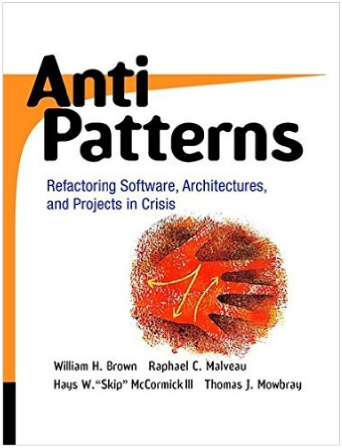
\includegraphics[width=0.6\textwidth]{bookCover.png}
	\end{minipage}%
\end{minipage}

\section{Семь причин провала проектов}

Авторы книжки про антипаттерны вделяют семь главных причин, по которым эти антипаттерны, собственно, вообще появляются в промышленном коде. Эти причины таковы.

\begin{itemize}
	\item Спешка --- пожалуй, самая главная причина появления плохого кода. Бывает тяжело думать над правильным и архитектурно красивым решением, если завтра релиз, а ещё не поправлен десяток критических багов. Проблема в том, что промышленная разработка почти всегда ведётся в спешке, и на это есть простые экономические причины --- если у программистов есть время делать хорошо и правильно, они могли бы потратить это время на то, чтобы сделать больше фич или сдать больше проектов, поэтому никто, кроме самих программистов, не заинтересован в качестве кода. Заказчику не нужна архитектура, ему нужен работающий продукт. И если даже иногда оно будет вести себя странно, это тоже может быть некритично --- пользователь перезапустит приложение, и всё. Из-за этого растёт технический долг --- вы думаете, что завтра релиз и послезавтра вы перепишете все костыли, что сейчас навставляли, но послезавтра новый релиз через две недели, на вас уже написали задач, с которыми вы чувствуете, что справитесь только недели через три, и цикл повторяется. И получение позитивной обратной связи в виде довольного менеджмента и заказчика только ухудшает ситуацию.
\end{itemize}

\end{document}
